\chapter{Implementation}\label{chap:impl}

\section{Environment}

\subsection{The \ttmcfw}

\ttmc\ is an extensible, configurable verification framework developed by the \bmemit\ that offers model checking algorithms for various models, such as programs and statecharts. The models are described by domain specific languages, and translated to common formalisms, including the state transition system, the control flow automaton, and the timed automaton. Besides formalisms, abstract domains and frameworks for common model checking approaches are also implemented. \ttmc\ uses an SMT solver called \textsc{Z3}\footnote{https://github.com/Z3Prover}, that is able to recognize various first order theories, such as difference logic.

I have decided to extend the \ttmcfw\ with the presented configurable framework for model checking timed automata. The implemented framework relies on the model checker's extended timed automaton representation: the \emph{Timed Control Flow Automaton}, Z3 interface, and a modified version (modifications described in Chapter \ref{chap:timed_cegar}) of the zone implementation described in \cite{bengtsson2004timed}.

\subsection{Achitecture}

\begin{figure}
	\centering
	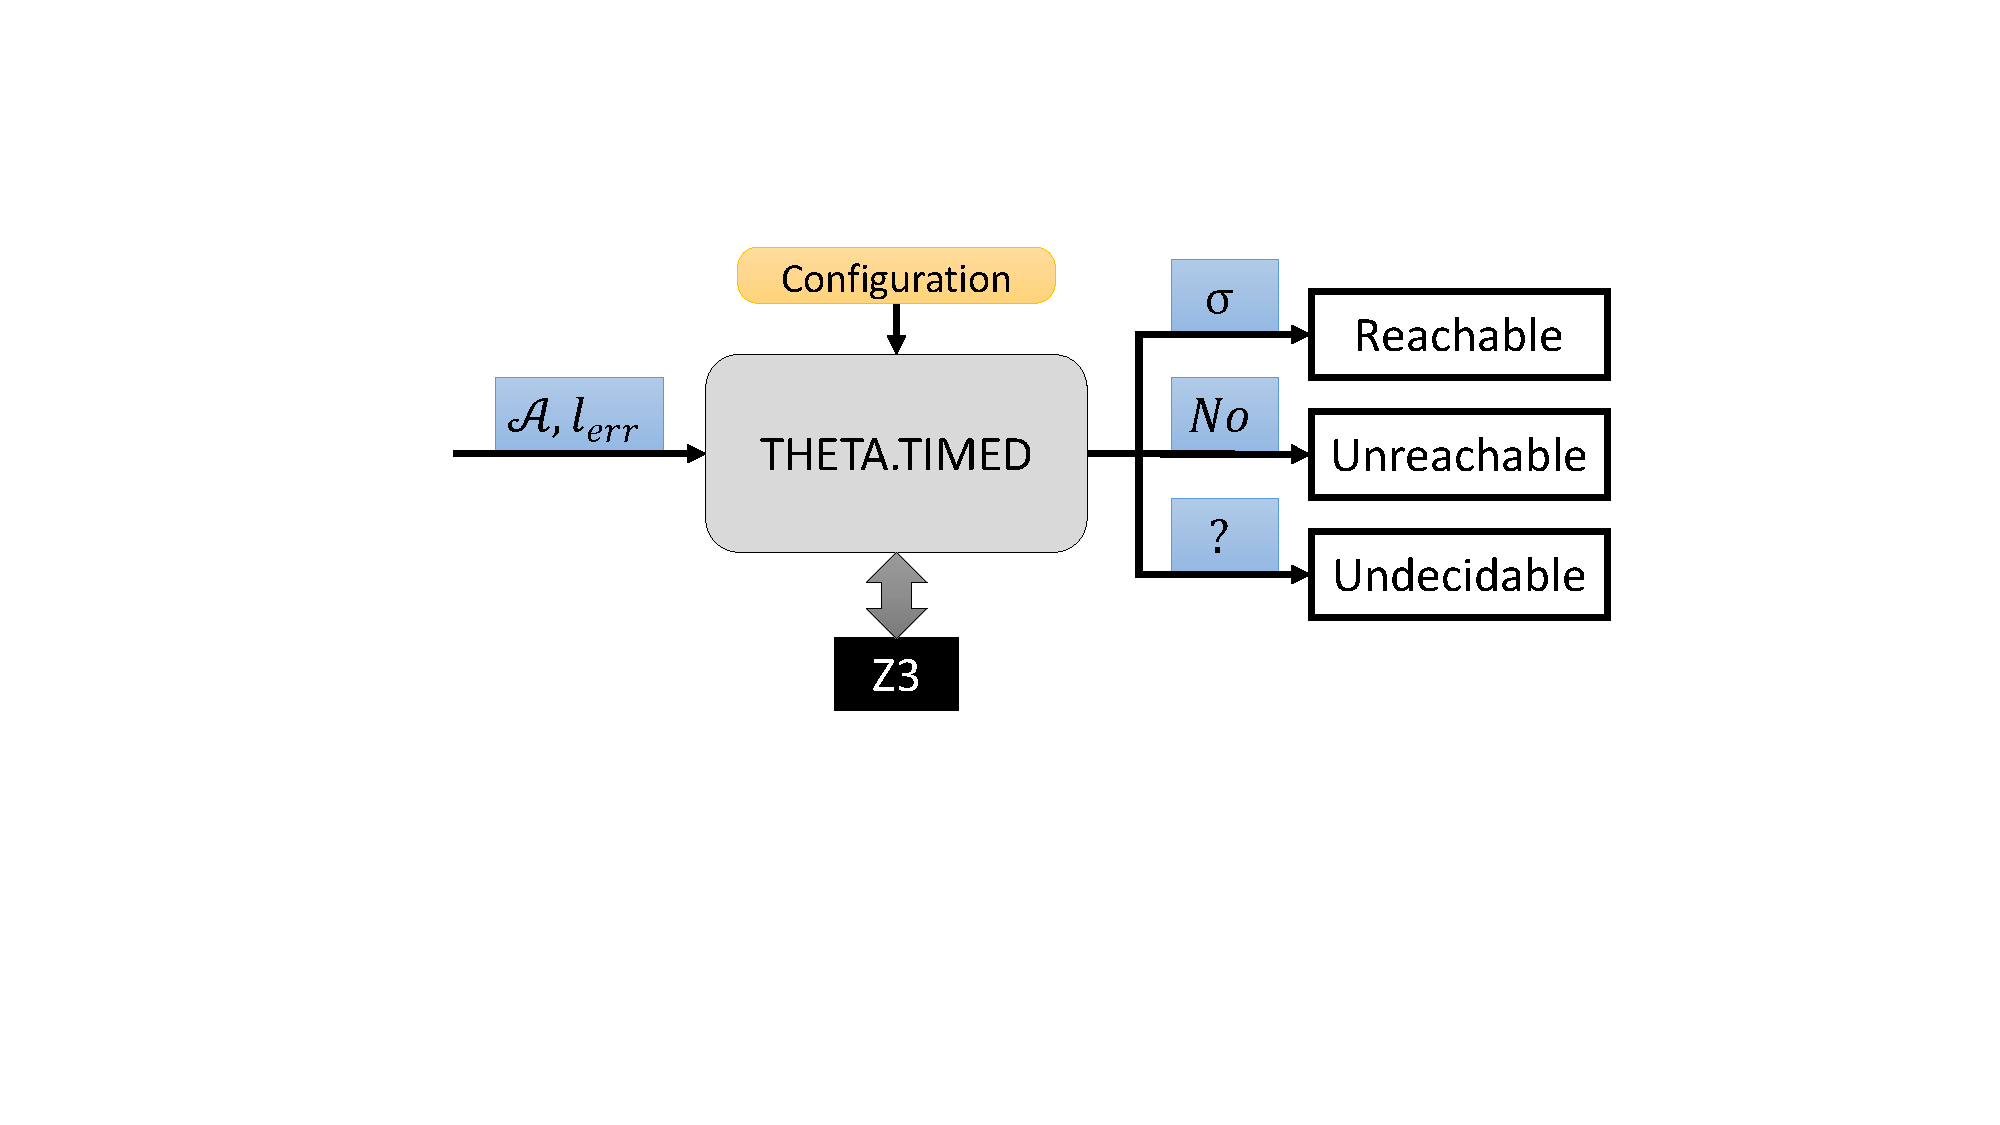
\includegraphics[width=.7\textwidth]{include/figures/architecture}
	\caption{Basic architecture of the framework}
	\label{fig:arc}
\end{figure}

The basic architecture of the framework presented in Chapter \ref{chap:timed_cegar} is shown in Figure \ref{fig:arc}.

The input of the algorithm consists of an input of the problem (a timed automaton $\mathcal{A}$ and a location $l_{err} \in L(\mathcal{A})$), and a configuration of the algorithm: compatible implementations of the CEGAR phases, and their parameters (e.g. the bound of the bounded model checker).

The output of the algorithm can be an execution trace by which $l_{err}$ is reachable, \emph{No} if $l_{err}$ is unreachable, or \emph{Undecided}. The latter case can happen for two causes: either the computations on the discrete variables make the problem undecidable, or the bounded model checker proved that $l_{err}$ is unreachable in the given number of steps. 



\section{Measurements}

The goal of the measurements is to evaluate the designed algorithm's performance and scalability, and draw conclusions about what combination of algorithms are efficient. The inputs are scalable automata chosen from Uppaal's benchmark data\footnote{https://www.it.uu.se/research/group/darts/uppaal/benchmarks/}. Uppaal supports extensions of the timed automaton formalism (network automata with synchronization channels) that are not implemented in the \ttmcfw, but can be transformed to the timed control flow automata formalism. This transformation was performed before the measurements.

Measurements were performed on a personal computer with a 2.60 GHz core i5 processor. The program was operating on a maximum of 4GB memory, however, this was not fully used, as it was the solver that run out of memory in most cases.
%\todo{Célok ismertetése, mérések bemutatása. Mit akarunk mérni, mivel fogjuk összehasonlítani, milyen bemeneteken, és miért.}

\subsection{Inputs}

This section describes the input models used for measurements. These models are widely used in benchmarks of timed automata-related algorithms.

\subsubsection{Fischer's protocol}

\begin{figure}
	\centering
	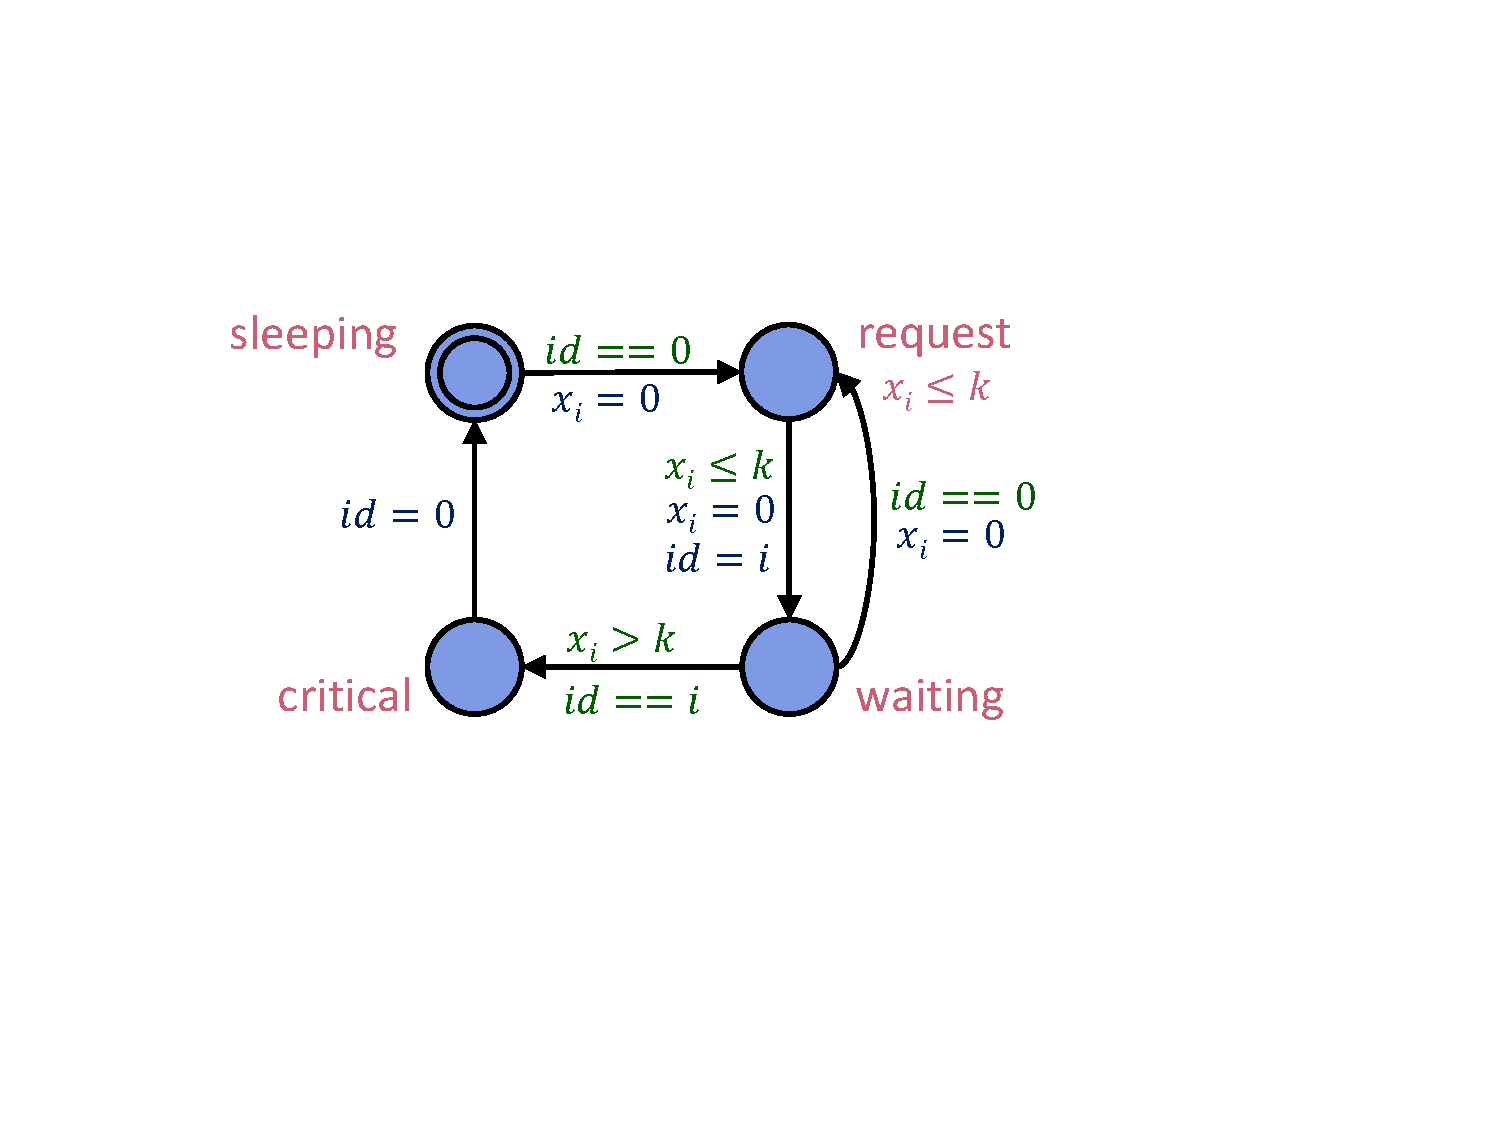
\includegraphics [width=0.5\textwidth]{include/figures/fischer_figure}%
	\caption{Fischer's protocol}
	\label{fig:fischer}
\end{figure}  

Fischer's protocol assures mutual exclusion by bounding the execution
times of the instructions. It can be applied to a number of processes accessing a
shared variable. Figure \ref{fig:fischer}  shows the operation of a process.
The location \emph{critical} indicates that the process is in the critical
section. The value of the shared variable $id$ ranges between 0 and $n$,
where $n$ denotes the number of processes. The model also contains a 
clock variable $x_i$ for each process where $i \in \{1 \ldots n\}$ denotes the
identifier of the process. The constant $k$ is a parameter of the automaton.

The examined property (mutual exclusion) can be formulated as an input of the reachability problem, where the system is network of $n$ instances of the depicted automata and the reachable states are when at least two of them are in the critical section. 

\subsubsection{CSMA/CD protocol}

Carrier sense multiple access with collision detection (CSMA/CD) is a media access control method used in Ethernet technology. The stations are communicating through a medium that can only maintain one transmission. They can sense if the medium is busy, but there is a certain amount of propagation delay (denoted with $\sigma$), so it is possible that another station started transmission since the last information, and collision can occur. In this case the medium broadcasts a jam signal, and the stations pick a random time between 0 and $2\sigma$ time units to try transmission again.

The examined property (collision detection) can be formulated as an input of the reachability problem, where the system consists of one medium and $n$ stations ($n \geq 2$) and the reachable states are when at least two of them are transmitting and at least one of them has been transmitting since at least $2\sigma$ time units -- i.e. the collision was not detected.

\subsubsection{Token ring FDDI protocol}

Token ring and FDDI protocal are actually two distinct protocols, that are based on the same idea: a ring network of server stations, with a token travelling around the ring. The server owning the token is allowed to communicate, but only within certain time limits to ensure fairness: first, synchronous transmission happens, that is only allowed for at most \emph{sa} time limits (\emph{sa} is the previously agreed timebound of synchronous communication) and then assynchronous transmission can happen until the station exceeds \emph{ttrt}, which is the \emph{tartget token rotation time}: the time passed since the previous transmission of the same station.

The examined property (token exclusiveness) can be formulated as an input of the reachability problem, where the system consists of one token ring and $n$ stations ($n \geq 2$) and the reachable states are when at least two of them are owning the token.

\subsection{Results}

This section presents the performed measurements and their results.

\subsubsection{Token ring FDDI measurements}

The Token ring protocol is a special input, since the examined safety property can be proven solely based on the structure of the automaton, thus the analysis of the initial abstraction is able to prove the property and refinement is not necessary. This proves how useful abstraction is, but the measurements on this automaton can only compare the efficiency of the pathfinding algorithms, that are almost the same in all presented algorithms (breadth-first search and depth-first search).

\begin{figure}
	\centering
	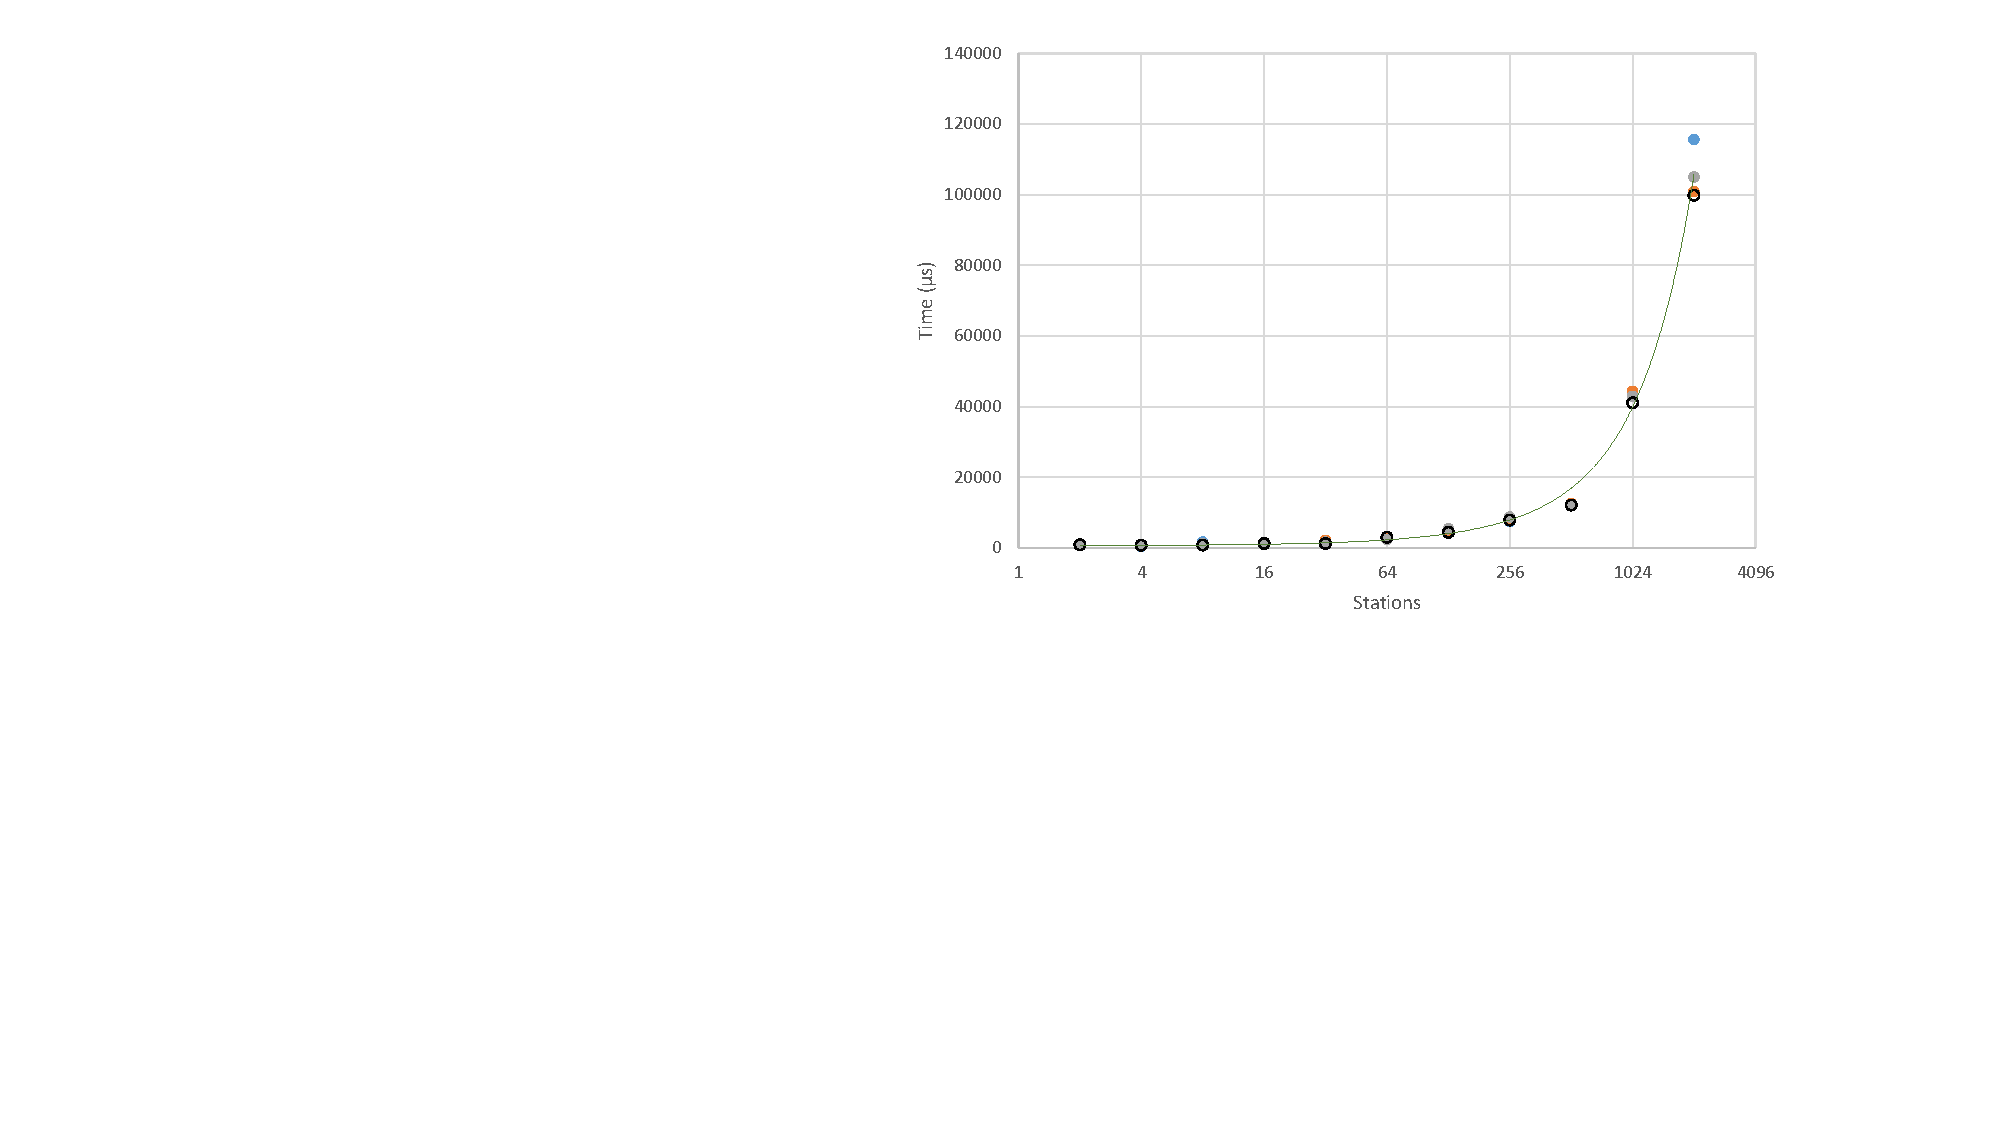
\includegraphics[width=\textwidth]{include/figures/diag_tokenfddi}
	\caption{Results of measurements on the token ring example}
	\label{fig:tokendiag}
\end{figure}

The algorithms were executed on the timed automata representations of token rings consisting of $2^n$ stations ($2 \leq n \leq 11$), and their execution times were measured. Each algorithms on each input was run 15 times and the average the execution times was calculated. The results are depicted in Figure \ref{fig:tokendiag}. The execution times were roughly the same, all in $\mathcal{O}(n^2)$, as it is expected from pathfinding algorithms, however, these measurements did not include the algorithm that uses a bounded model checker.

\subsubsection{Bounded model checker measurements}

The algorithm that uses a bounded model checker can not be compared to the other algorithms, because it scales with different characteristics. To demonstrate this I have executed the algorithm with on token ring protocol of different sizes, 15 times each and calculated the average runtime. The bound was set to 50 each time.

\begin{figure}
	\centering
	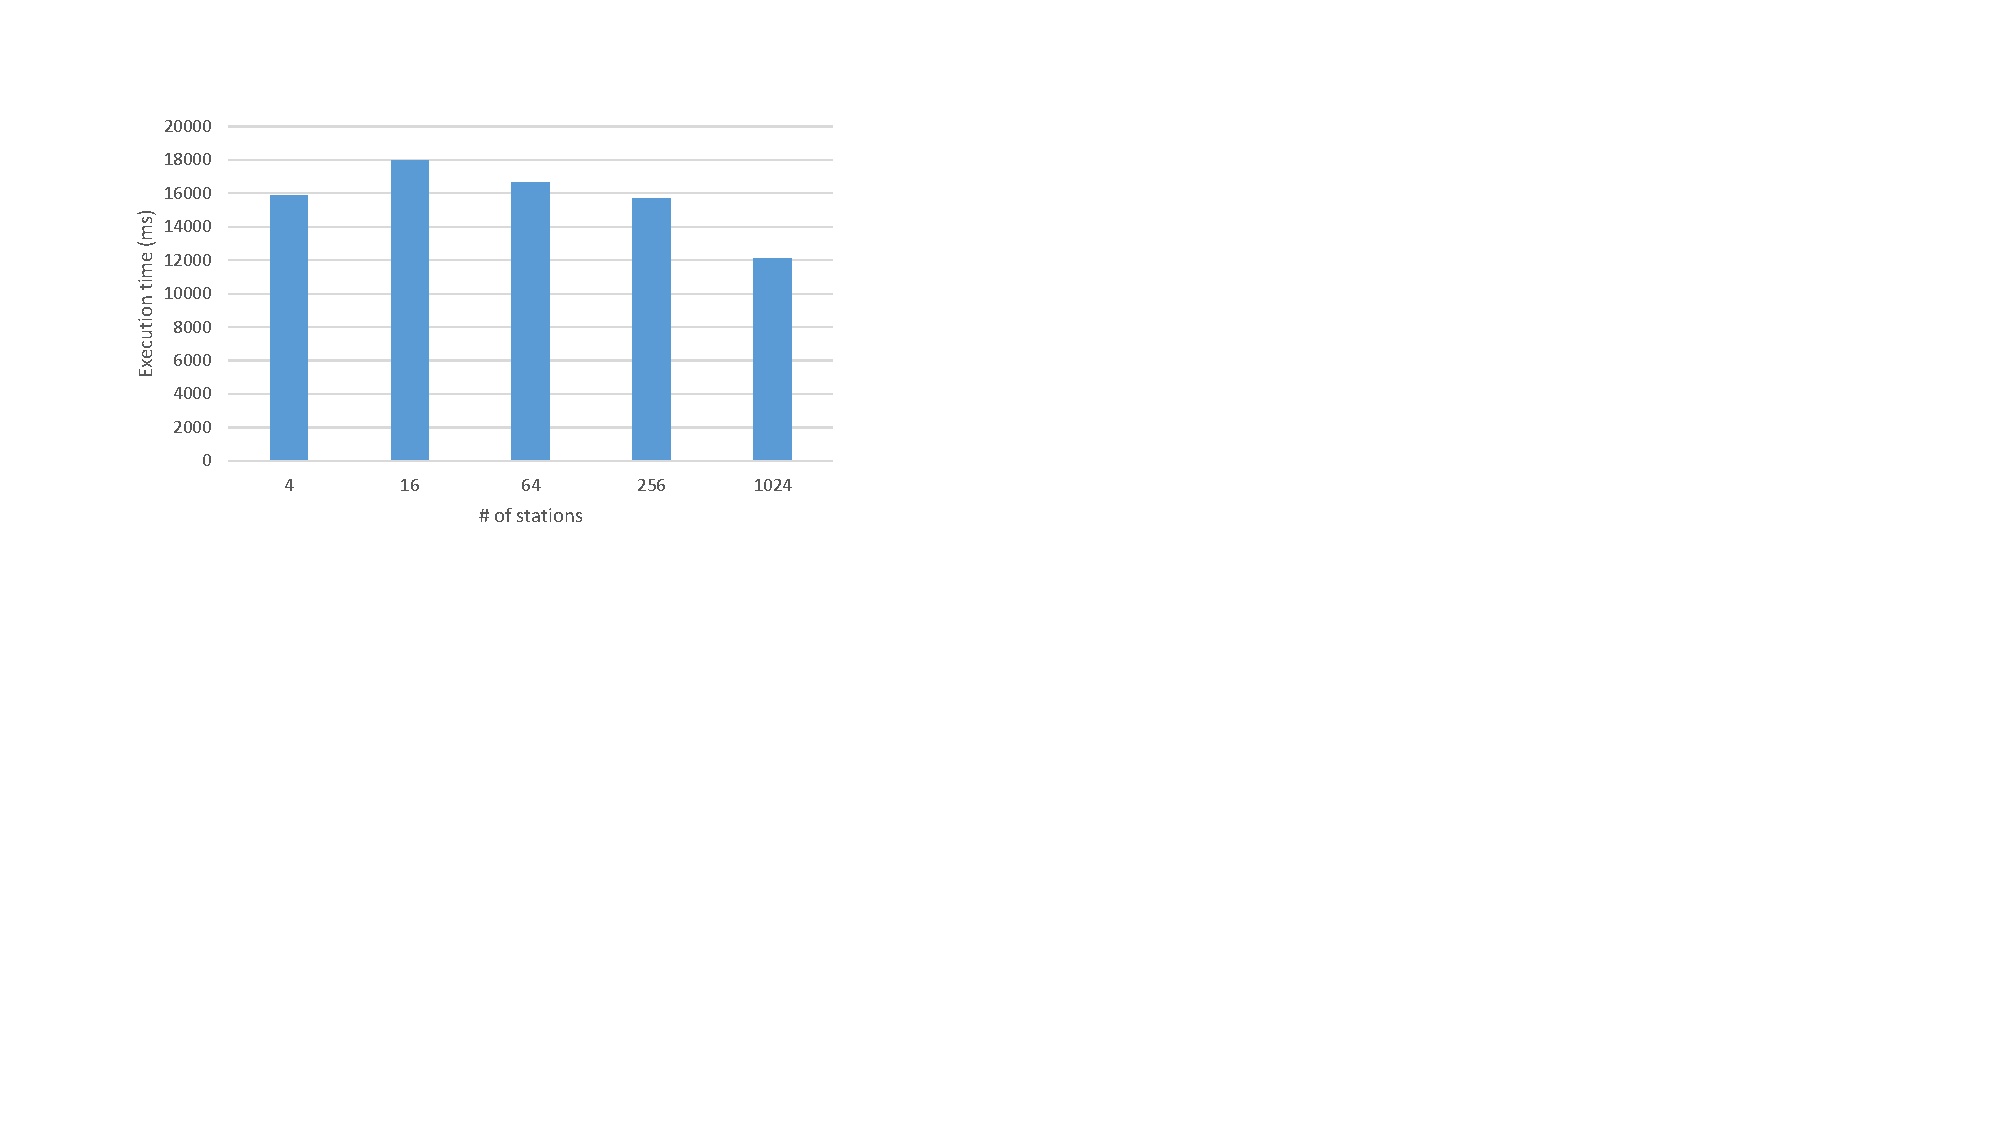
\includegraphics[width=\textwidth]{include/figures/diag_bound_station}
	\caption{Results of measurements with different number of stations}
	\label{fig:tokenboundstations}
\end{figure}

Figure \ref{fig:tokenboundstations} depicts the result of the measurements. It can be seen, that the execution times do not grow (although it is interesting how the execution times decrease -- this is probably caused by some environmental characteristics). On the other hand, the bound has a great influence on the runtime. To demonstrate this, I have executed the algorithm with different bound values on the timed automaton model of the token ring of three stations -- 15 times each. The bound varied between 5 and 50.

\begin{figure}
	\centering
	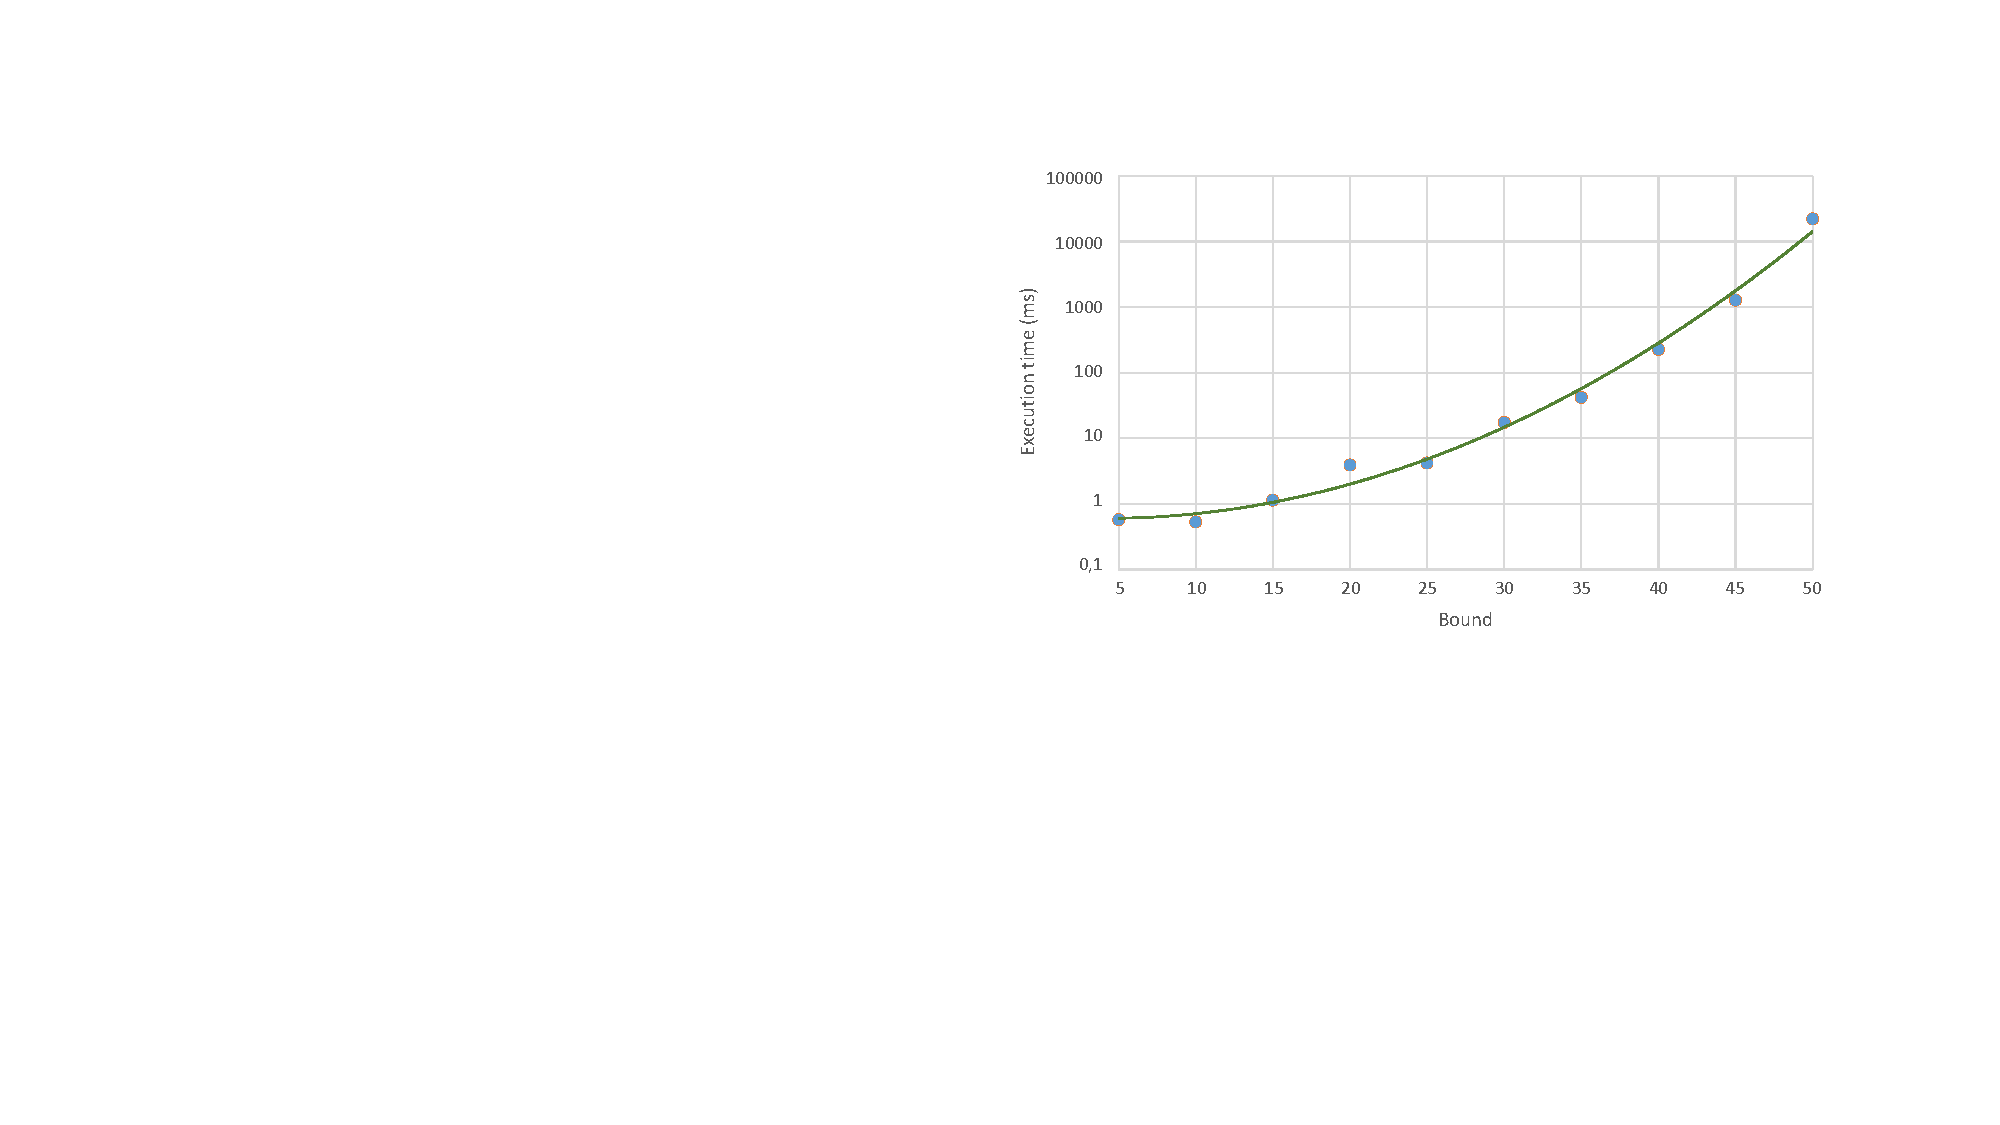
\includegraphics[width=\textwidth]{include/figures/diag_bound}
	\caption{Results of measurements with different bounds}
	\label{fig:tokenbound}
\end{figure}

The results of the measurements are depicted in Figure \ref{fig:tokenbound}. The scale on the vertical axis is logarithmic, and the trendline is parabolic. This means that the complexity of this algorithm is greater, than exponential in the value of the bound.

\subsubsection{Measurements on Fischer and CSMA/CD protocols}

The other algorithms were measured on timed automata representations of Fischer and CSMA/CD protocols, six times each. Memory problems occured at the Fischer protocol of four processes and the CSMA/CD protocol of five stations. One of the algorithms couldn't run on the CSMA/CD protocol of four stations either.

\begin{figure}
	\centering
	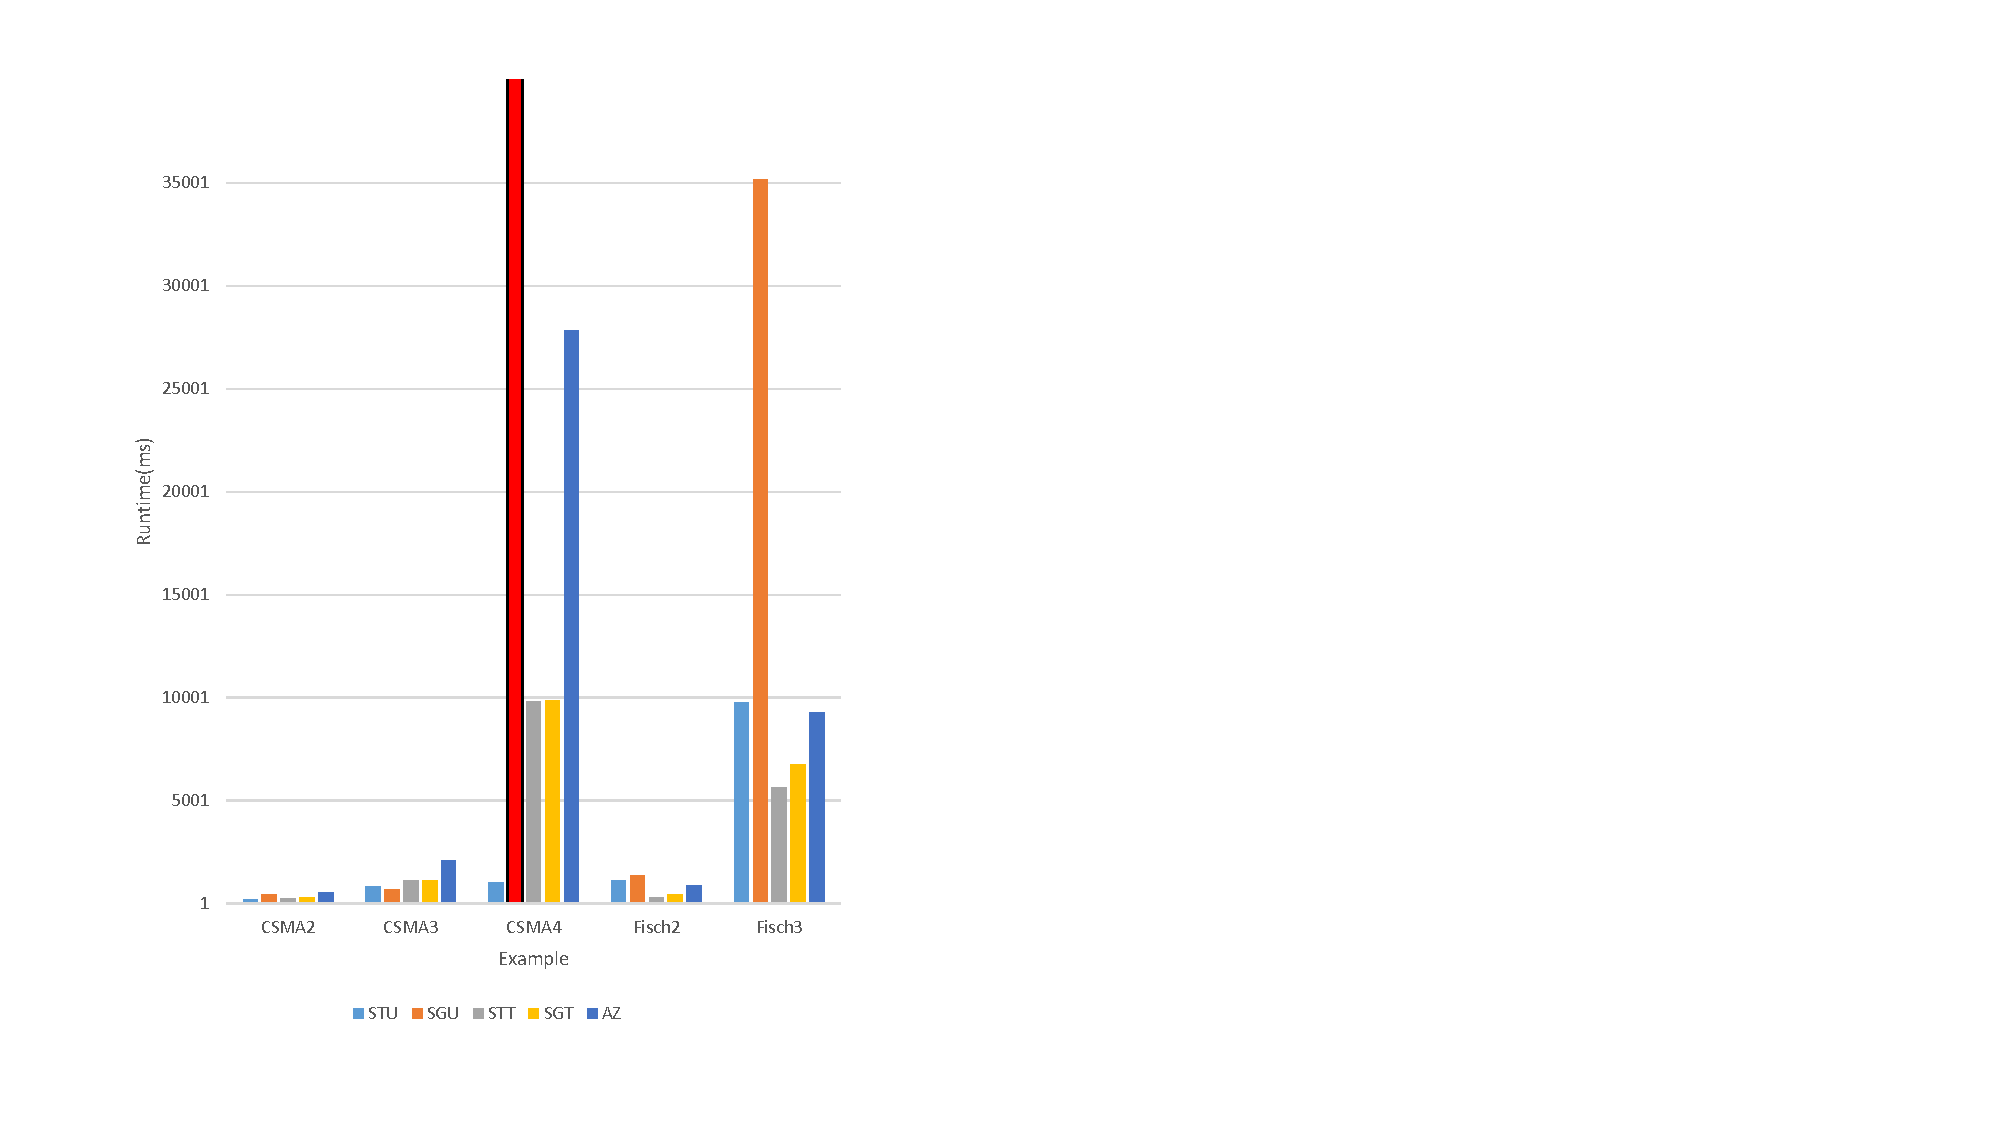
\includegraphics[width=\textwidth]{include/figures/diag_fischcsma}
	\caption{Results of measurements on Fischer and CSMA/CD protocols}
	\label{fig:mesurements}
\end{figure}

The results of the measurements are depicted in Figure \ref{fig:mesurements}. The models are denoted by Fisch$n$ and CSMA$n$ for the Fischer protocol and the CSMA/CD protocol of $n$ participants, respectively. The abbreviations denote the algorithms, that are composed the following way:

\begin{itemize}
	\item AZ denotes abstraction-based refinement with zone graph exploration
	\item STU denotes state space-based refinement operating on the tree representation of the abstract zone graph where the precisions of the zones are based on the unsat core of the trace,
	\item SGU denotes state space based refinement operating on the graph representation of the abstract zone graph where the precisions of the zones are based on the unsat core of the trace,
	\item STT denotes state space-based refinement operating on the tree representation of the abstract zone graph where the precisions of the zones are based on the trace activity, and
	\item SGT denotes state space based refinement operating on the graph representation of the abstract zone graph where the precisions of the zones are based on the trace activity.
\end{itemize}

The algorithm denoted by SGU run out of memory when executed on the timed automaton representation of four stations communicating with CSMA/CD protocol -- hence the red colour.

\subsection{Evaluation}

The performed measurements are not exhaustive, thus one should not come to far-reaching conclusions. However, there are some observations worth mentioning.

From the CSMA/CD examples it can be concluded that automaton-based refinement (algorithm AZ) does not scale well. The cause of this can be explained by considering automaton based refinement as a special case of state space-based refinement where the calculated precision assigns the same set of clock variables to each node, and that refines the complete graph not just a trace. Automaton based-refinement recovers so much of the hidden information that it prevents efficient model checking.

Out of the algorithms with state space-based refinement, the ones denoted by STT and SGT seem to perform better than the others. STT may be a bit more efficient, but their results are roughly the same. This is surprising, because the abstract state space representation is different in the two algorithms, and many of the techniques used in the algorithm are representation-dependent. It is interesting that the efficiency of two algorithms using different graph representations is almost the same.

Algorithm STU performs well on the CSMA/CD inputs, but this does not seem to be the case for the Fischer examples. However, it is worth mentioning that STU is the only algorithm that has been successfully ran on the Fischer protocol of four participants in the performed measurements. On the other hand, algorithm SGU hasn't performed well on either type of the test cases.

In conclusion, out of the presented algorithms STT seems to be the most efficient, and SGU seems to be the least efficient one. Measurements also suggest that state space based refinement may be generally more efficient than automaton based refinement.


%\subsection{Evaluation}

%\todo{Miérések eredményének összesítése, mit tudtunk meg ebből.}

